\documentclass[a4paper,10pt]{article}
\usepackage[T2A]{fontenc}
\usepackage[utf8x]{inputenc}
\usepackage{ucs}
\usepackage{cmap}
\usepackage[english,russian]{babel}
\usepackage{amsmath}
\usepackage{color,graphicx}

\title{Заголовок}
\author{Автор}

\begin{document}


\begin{center}
\thispagestyle{empty}
\centering
\ \\
\ \\
\ \\
\ \\
\ \\
\ \\
\ \\
\ \\
\ \\
\textsc{\Large Мотивационное письмо}\\[1cm]
\ \\
\ \\
\ \\
\ \\
\ \\
\ \\
\ \\
\ \\
\ \\
\ \\
\ \\
\ \\
\ \\
\ \\
\ \\
\ \\
\ \\
\ \\
\ \\
\ \\
\ \\
\ \\
\ \\
\ \\
\ \\
\ \\
\ \\
\ \\
\ \\
\ \\
\ \\
\end{center}
Чернышев Алексей, 2013

\newpage
\tableofcontents
\newpage
\setlength{\parindent}{10pt}

\section{Вводные слова}
Основная задача будущего исследования -- создать унифицированный подход в использовании возможностей сложных динамических нейроннных систем в проблемах обработки больших объемов данных и осуществления при помощи них классических задач машинного обучения таких как кластеризация, регрессия, классификация.\\
\indent Динамические системы вдохновленные структурой коры головного мозга давно являются, как минимум, любопытным феноменом для учёных. Мозг является сложным многосистемным вычислительным устройством, который поражает своими вычислительными способностями и подчерпнуть хоть немного из его строения, научиться это использовать, является большим вызовом.

\section{Машинное обучение, основные проблемы}
\label{sec:ml}
Одной из классических задач машинного обучения является найти зависимость между скрытыми переменными (причиной) и данными (следствием). С такой задачей машинное обучение уже давно с успехом справляется. Можно взять в качестве примера наивный байесовский классификатор, в котором делается предположение о независимости признаков друг от друга (то есть скрытые переменные не взавимосвязаны причинно-следственной связью) и в итоге получить классификатор, который будет классифицировать объекты с той или иной погрешностью.\\
\indent Основная проблема подобного подхода в том, что в реальных сложных задачах мы почти никогда не встретим случая, когда данные порождены абсолютно независимыми причинами.\\
\indent Существуют графические вероятностные модели \cite{prob_graph} в которых подобные зависимости вводятся в виде графа факторов. Также существует много способов обучать такие модели, но так или иначе, все они сталкиваются с невозможностью описать зависимость всех факторов друг от друга. Если, например, рассмотреть в качестве данных картинку 32x32, в которой каждый пискель принимает значение $\{0,1\}$, то, чтобы описать зависимость всех факторов друг от друга, необходимо ввести $2^{1024}$ дополнительных факторов, не говоря о том, как сложно их обучить.\\
\indent В 2003 году, B. Taskar предложил способ обучения графической модели, которая может учитывать попарно связанные факторы \cite{taskar}, но тем не менее задача как рассматривать более высокоранговые связи внутри данных всё также остра.
\section{Reservoir computing}
\label{sec:res_comp_sec}
Почти одновременно и с большой помпой вышли две работы H. Jaeger \cite{esn} и W. Maass \cite{lsm} в 2004 г., описывающие модели \textit{Echo State Networks} и \textit{Liquid State Machine} соотв., которые положили начало новому взгляду на использования рекуррентных сетей . Рекуррентные сети не без успеха использовались и до выхода работ, но рекуррентность в сетях порождают труднопреодолимые проблемы, как нестабильность и проблема обучения таких сетей \cite{rnn_prob}.\\
\indent Успех вышеназванных работ заключатся в уникальном по простоте подходу к динамическим системам (см. рис~\ref{res_comp}).
\begin{figure}[ht]
\centering
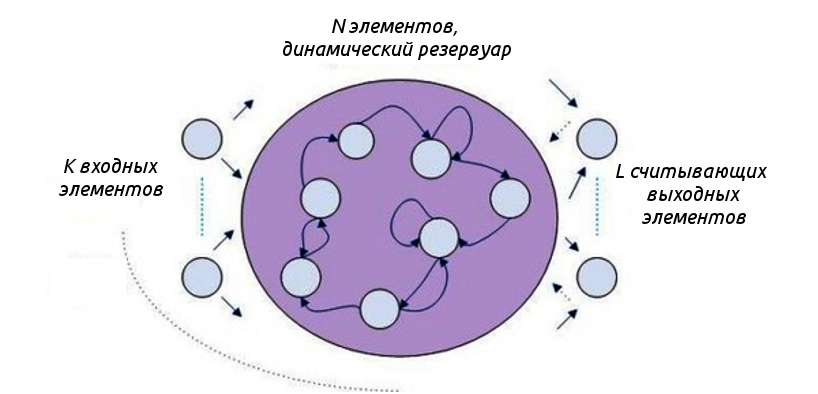
\includegraphics[width=1\linewidth]{res_comp}
\caption{схема Reservoir Computing}
\label{res_comp}
\end{figure} \\
\indent Основной принцип работы модели в том, что вычислительный резервуар, который представляет собой динамическую рекуррентную нейронную сеть, принимает уникальное состояние для каждого элемента данных, выходные же элементы по средством настраиваемых весов, обучаются на состояниях резервуара.\\
\indent Методы обучения считывающих (\textit{readout}) элементов на состояниях резервуара могут быть самыми примитивными -- используя только решение системы нормальных уравнений для регрессии методом наименьших квадратов, уже можно добиться хороших предсказательных способностей \cite{esn_site}.\\
\indent Примечателен тот факт, что веса связей между элементами резервуара во время обучения остаются постоянными. 
\section{Нейронные сети, тренд развития}
Первое поколение Искусственных Нейронных Сетей (ИНС) взяло только основные принципы работы биологических нейросетей. В них нейрон формализован как сумматор принимающий на вход сигналы от других нейронов и на основе искусственно введенной нелинейности решает передавать сигнал дальше или нет.\\
\indent Вторым поколением ИНС можно назвать модели школы \textit{Deep Learning}, которую основал J. Hinton с выходом работы \cite{hinton2006}. Эти модели имеют стохастическую природу - нейрон передает или не передает сигнал в зависимости от вероятности выражаемой через коэффициенты модели, которые обучаются на данных без учителя.\\ 
\indent Обучение без учителя является ключевым показателем интеллектуальности алгоритма. Интеллект сам по себе, как свойство живых организмов, представляет собой следствие самоорганизации природы в определенных условиях \cite{evolut}. Руководствуясь подобными предпосылками, на базе школы \textit{Deep Learning} выросло направление в \textit{Machine Learning - Representation Learning} \cite{yoshua}.\\
\indent \textit{Representation Learning} собрал для себя следующие принципы, которые, по большей части, взяты именно из особенностей работы мозга:
\begin{itemize}
\item распределенность хранения (distributed representation);
\item разреженность представления (sparse code);
\item генеративные модели (generative models);
\end{itemize} 
\indent \indent Стоит заметить, что \textit{Deep Learning} привнес новый взгляд на пробему решения вопроса обучения больших полносвязанных графических моделей. В своих работах Hinton применяет современные методы цепей Монте-Карло, направляя сэмплированные частицы (\textit{particles}) по направлению градиента поверхности правдоподобия модели. К сожалению его метод обучения ограничен только определенным классом моделей.\\
\indent Как итог небольшого экскурса в историю ИНС, невооруженным вглядом можно заметить, что общий тренд их развития стремительно идёт по направлению к биоподобным моделям.
\section{Новости с фронтов Neuroscience}
\label{sec:neuroscience}
Начиная с создания динамической модели аксона кальмара в работе Hodgkin и Huxley \cite{hodhux}, в 50-ых сформировалась научная область изучающая поведение динамических систем и приведение их в соответствие с наблюдаемыми данными - \textit{Computational Neuroscience}. Развитие компьютеров позволяют всё больше и больше понять тонкости взаимосвязи химических реакций в мозгу.\\ 
\paragraph*{Neural Coding.} До 90-ых в сообществе учёных была твёрдая уверенность, что информация в нейронах кодируется при помощи спайковой интенсивности (\textit{rate coding}). В работе D. Warland \cite{time_cricket} измерили временные статистики спайковой активности сверчка, на усы которого воздействали слабым потоком воздуха, выяснилось, что нейронная активность наиболее всего коррелирует с временем между спайками. Также, работе J. Gautrais \cite{time_code} показал, что потенциальное количество информации закодированной нейросетью растет экспоненциально с ростом количества нейронов, если информация кодируется при помощи временной разницы между спайками.\\
\paragraph*{Dendritic Computation.}
Роль дендритов много времени не была ясна и им не уделяли много внимания: многие симуляции организовывали вовсе без дендритов - синаптические связи подключали напрямую к клетке. В 2003 году появилась работа \cite{dendr0}, где показывается нелинейность поведения дендритов и феномена появления, так называемого, кластера синапсов. Здесь \cite{dendr1} рассказывается, что используя только сеть дендритов и один нейрон была создана сеть распознающая лица.\\
\paragraph*{Synaptic Plasticity.}
Пластичность синапсов, как ключ к обучаемости и интеллекту всегда был интересен ученым в Neuroscience и не только. Начиная с 1998 года появилась, уже классическая, модель пластичности синаптических связей \cite{syn0} \textit{Spike Timing Dependence Plasticity} (\textit{STDP}). Она во многом солидарна со правилом Хэбба \cite{hebb}, предсказанным им ещё в 1949 году -- связи между нейронами, которые активны большую часть времени, усиливаются, однако правило не учитывает момент ослабления синаптических связей. Современное правило пластичности синапсов, биологически верное, построено на разнице во времени спайков pre-нейрона и post-нейрона. Если pre-нейрон произвел спайк, а потом произвел спайк post-нейрон, то синаптическая связь между pre-нейроном и post-нейроном усиливается. Если же post-нейрон произвел спайк раньше, чем pre-нейрон, то связь ослабляется. Модель, наиболее натурально описывающая этот феномен -- экспоненциальная.\\
\indent Существует множество работ \cite{syn1, syn2, syn3}  доказывающих, что рекуррентные сети, обучающиеся на таком правиле способны к самоорганизации и кластеризации.

\paragraph*{Polychronious Groups.}
Как гипотеза, в работе Eugene Izhikevich \cite{izh_groups}, была предложена идея работы мозга на основе полихронов -- особых груп нейронов, которые имеют место формироваться в больших симуляциях нейронных сетей (около $10^5$ нейронов). Полихронные группы формируются в больших количествах и в разных качествах, есть группы временные, которые умирают сразу, есть постоянные, но также есть определенные виды групп которые соответствуют определенному входному паттерну \cite{patt_groups}.

\section{Основная гипотеза}
Вместо того, чтобы порождать огромное множество различных алгоритмов машинного обучения для каждого конкретного случая зависимости факторов (секция \ref{sec:ml}), предпологается создать на базе \textit{Reservoir Computing} (секция \ref{sec:res_comp_sec}) один специальный сложный алгоритм, который обучается на корелляционных атрибутах нейронной активности.\\
\indent Гипотеза подразумевает существование единого принципа работы когнитивных функций мозга и возможности в большей или меньшей  степени приблизить принцип работы резервуара с динамической нейронной сетью к этому единому природному принципу, что как следствие, предпологает наличия у резервуара свойств обнаружения сложных зависимостей в данных, которые кодируются в том или ином виде.

\section{Задача и модель для проверки гипотезы}
В качестве задачи предлагается задача обработки большого корпуса текстов. Результат обработки будет в выделении наиболее вероятной тематики текста (\textit{Topic modeling}). Этой задаче присуще сложные внутренние зависимости среди скрытых переменных, которые образуют смысл текста.\\
\indent Чтобы решить данную задачу необходимо решить отдельные подзадачи относительно каждой части модели:\\
Входные элементы:
\begin{itemize}
\item Найти наиболее оптимальный способ представления текста во входных элементах. Предлагается начать со схемы, где каждый входной элемент ответственнен за определенный слог \cite{rnn_text};  
\item Найти оптимальный размер порции текста и наиболее оптимальное время <<чтения>> резервуара этой порции;
\end{itemize} 
Резервуар:
\begin{itemize}
\item Создать наиболее оптимальную структуру резервуара, с т.з. обучения и хранения информации. Предлагается осуществлять это при помощи методов из Теории Информации \cite{inf_th}; 
\item Выбрать наиболее оптимальную структуру резервуара. Предлагается начать с модели работ Izhikevich \cite{izh_groups} и постепенно усложнять её различными вариациями, частично описанных в секции \ref{sec:neuroscience};
\end{itemize}
Выходные элементы, метод обучения. Предлагается использовать два подхода к обучению, которые сочетают различные аспекты решения задачи:
\begin{itemize}
\item Обучение с учителем. Для обучения предлагается использовать структурный метод опорных векторов, в качестве дополнительной ограничивающей структуры ввести кросс-зависимости на полихронные группы нейронов (\textit{Polychronius groups});
\item Обучение без учителя. Предлагается использовать модель Айзинга (\textit{Ising models}) из физики, которая успешно применяется в раскодировании нейронной активности \cite{schneidman0, schneidman1}, и обучать её вариационным методом из \textit{Deep Learning} -- \textit{Contrastive Divergence}\cite{hinton2006};
\end{itemize} 

\section{Заключение}
Автор рассмотрел последние наработки в областях использования рекуррентных сетей, последние, наиболее близкие к биологическим характеристикам, модели \textit{Computational Neuroscience} и выработал естесственное продолжение в сторону усложнения моделей \textit{Reservoir Computing} с целью создать перспективный подход в обработке больших данных с внутренними кросс-зависимостями.\\
\indent Также стоит отметить, что дополнительным итогом исследовательской работы может стать новое понимание работы когнитивных функций мозга, что может открыть новые горизонты работ в разработке интеллектуальных систем и алгоритмов для работ с ними.
\newpage
\addcontentsline{toc}{section}{Список литературы}
\begin{thebibliography}{9}
\bibitem{prob_graph}
D. Koller and N. Friedman, Probabilistic Graphical Models: Principles and Techniques,2009, MIT Press
\bibitem{taskar}
Max-Margin Markov Networks,  B. Taskar, C. Guestrin and D. Koller. Neural Information Processing Systems Conference (NIPS03), Vancouver, Canada, December 2003
\bibitem{esn}
Herbert Jaeger, Harald Haas; Harnessing Nonlinearity: Predicting Chaotic Systems and Saving Energy in Wireless Communication; 
Science 2 April 2004: Vol. 304 no. 5667 pp. 78-80 
\bibitem{lsm}
Maass, Wolfgang; Natschläger, Thomas; Markram, Henry (November 2002), "Real-time computing without stable states: a new framework for neural computation based on perturbations", Neural Comput 14 (11): 2531–60
\bibitem{rnn_prob}
Sepp Hochreiter; The Vanishing Gradient Problem during Learning; INTERNATIONAL JOURNAL OF UNCERTAINTY, FUZZINESS AND KNOWLEDGE-BASED SYSTEMS
\bibitem{esn_site}
http://minds.jacobs-university.de/mantas/code
\bibitem{hinton2006}
Hinton, G. E., Osindero, S. and Teh, Y. (2006)
A fast learning algorithm for deep belief nets.
Neural Computation, 18, pp 1527-1554
\bibitem{evolut}
Christoph Adami, Charles Ofria, and Travis C. Collier, Evolution of biological complexity (1997), PNAS 2000 97 (9) 4463-4468; doi:10.1073/pnas.97.9.4463
\bibitem{yoshua}
Yoshua Bengio, Aaron Courville, Pascal Vincent (2012), Representation Learning: A Review and New Perspectives, CoRR abs/1206.5538 
\bibitem{hodhux}
A. L. Hodgkin. A. F. Huxley. Chance and design in electrophysiology: an informal account of certain experiments on nerve carried out between 1934 and 1952. J Physiol, 263(1):1-21, Dec 1976.
\bibitem{time_cricket}
David Warland, Michael Landolfa, John P. Miller, William Bialek; Reading Between the Spikes in the Cereal Filiform Hair Receptors of the Cricket; Analysis and Modeling of Neural Systems; 1992, pp 327-333
\bibitem{time_code}
Jacques Gautrais, Simon Thorpe; Rate coding versus temporal order coding: a theoretical approach; 1998; Centre de Recherche Cerveau et Cognition UMR 5549, 133 route de Narbonne, 31062 Toulouse, France
\bibitem{dendr0}
Michael Hausser and Bartlett Mel.; Dendrites: bug or feature? Current Opinion in Neurobiology 2003, 13:372–383
\bibitem{dendr1}
https://class.coursera.org/bluebrain-001/class/index
\bibitem{syn0}
Guo-qiang Bi and Mu-ming Poo; Synaptic Modifications in Cultured Hippocampal Neurons: Dependence on Spike Timing, Synaptic Strength, and Postsynaptic Cell Type; The Journal of Neuroscience, 15 December 1998, 18(24): 10464-10472;
\bibitem{syn1}
Xiaoli Tao, Howard E. Michel. Data Clustering Via Spiking Neural Networks through Spike Timing-Dependent Plasticity. In Hamid R. Arabnia, editor, Proceedings of the International Conference on Artificial Intelligence, IC-AI 04, June 21-24, 2004, Las Vegas, Nevada, USA, Volume 1. pages 168-173, CSREA Press, 2004.
\bibitem{syn2}
Belatreche, Ammar and Paul, Rakesh (2012) Dynamic cluster formation using populations of spiking neurons. In: The 2012 IEEE International Joint Conference on Neural Networks (IJCNN), , Brisbane, Australia. IEEE. 6 pp.
\bibitem{syn3}
Bernhard Nessler, Michael Pfeiffer and Wolfgang Maass; STDP enables spiking neurons to detect hidden causes of their inputs; Computational, Information-Theoretic Learning with Statistics, Learning/Statistics \& Optimisation, Theory \& Algorithms; 2009
\bibitem{hebb}
Hebb, D. O. (1949). The Organization of Behavior: A Neuropsychological Theory. ISBN 978-0805843002.
\bibitem{izh_groups}
Eugene M. Izhikevich, Joe A. Gally, Gerald M. Edelman; Spike-Timing Dynamics of Neuronal Groups; (2004) Cerebral Cortex, 14:933-944
\bibitem{patt_groups}
Joseph Chrol-Cannon, Andre Gruning and Yaochu Jin; The Emergence of Polychronous Groups under Varying Input Patterns, Plasticity Rules and Network Connectivities; IJCNN The 2012 International Joint Conference on Neural Networks, 2012-06-10 - 2012-06-15, Brisbane, QLD
\bibitem{rnn_text}
Ilya Sutskever, James Martens, Geoffrey Hinton; Generating Text with Recurrent Neural Networks; ICML 2011. 
\bibitem{inf_th}
Borst A, Theunissen FE.; Information theory and neural coding; Nat Neurosci. 1999 Nov;2(11):947-57.
\bibitem{schneidman0}
Elad Schneidman, Michael J. Berry, Ronen Segev \& William Bialek; Weak pairwise correlations imply strongly correlated network states in a neural population; Vol 440|20 April 2006 doi:10.1038/nature04701
\bibitem{schneidman1}
Gasper Tkacik, Elad Schneidman, Michael J. Berry and William Bialeka; Ising models for networks of real neurons; arXiv:q-bio.NC/0611072 v1 22 Nov 2006


%\bibitem{izh_large}
%E. M. Izhikevich and G. M. Edelman. The Neurosciences %Institute,10640 John Jay Hopkins Drive, San Diego, CA, 92121.
%\bibitem{randall98}
%Randall C. O'Reilly, Six Principles for Biologically-Based Computational Models of Cortical Cognition, TRENDS IN COGNITIVE SCIENCES, 1998, 455--462
%\bibitem{hinton86}
%Hinton, G. E., McClelland, J. L., and Rumelhart, D. E. (1986)
%Distributed representations. 
%In Rumelhart, D. E. and McClelland, J. L., editors, Parallel Distributed Processing: Explorations in the Microstructure of Cognition. Volume 1: Foundations, MIT Press, Cambridge, MA.
%\bibitem{mcclel_rumer}
%McClelland, J. L., and Rumelhart, D. E. (1981). An interactive activation model of context effects in letter perception: Part 1. An account of basic findings. Psychological Review, 88, 375-407.
\end{thebibliography}

\end{document}
